\documentclass[a4paper,12pt,abstracton,titlepage]{scrartcl}
\usepackage{fancyhdr}
\usepackage[utf8]{inputenc}
\usepackage[T1]{fontenc}
\usepackage[top=2.5cm, bottom=2.5cm, left=2.5cm, right=2.5cm]{geometry}
\usepackage[affil-it]{authblk}
\usepackage{lipsum}
\usepackage[hidelinks]{hyperref}
\usepackage{graphicx}

% code for generating glossary, from http://tex.stackexchange.com/a/5837/59718
\usepackage[acronym,toc]{glossaries}
\newcommand{\dict}[2]{%
  \newglossaryentry{#1}{name=#1,description={#2}}%
  \glslink{#1}{}%
}
\makeglossaries

% Here we set up the header, meta-information and front matter
%\date{}      %// Today's date will appear when this is commented out.
\newcommand{\version}{0.1}

\author{Maarten Baertsoen and Daniel S. C. Schiavini}
\affil{Open Universiteit Nederland, faculteit Informatica \\
	T61327 - Afstudeerproject bachelor informatica}
\title{Planning}
\subtitle{Useful feedback in the\\ Ampersand parser}
\publishers{Version \version}

\pagestyle{fancy}
\lhead{M. Baertsoen and D.S.C. Schiavini}
\rhead{ABI Planning}
\cfoot{\thepage}
\setlength{\headheight}{15pt}

% Now the document starts
\begin{document}
\maketitle
\newpage

\tableofcontents
\listoffigures
\clearpage

\section{Introduction (R-M)}
\subsection{Identification}
This document contains the planning for the execution of the graduation project ``Useful feedback in the Ampersand parser''.
This planning gives the high-level requirements, the risks and a timefor the project.
As such, the planning provides the steps for reaching the project objectives, and provides criteria that are used to validate and accept the results of the graduation.

This document is part of the graduation project of the computer science bachelor at the Open Universiteit Nederland.
The project ``Useful feedback in the Ampersand parser'' is assigned to the students Daniel Schiavini and Maarten Baertsoen, with support of the supervisor Dr. Bastiaan Heeren and examiner Marko van Eekelen.
The assignment is given by professor Stef Joosten, who researches how to further automate the design of business processes and information systems by the development of the Ampersand project.

\subsection{Goal of this document}
The main goal of this document is to capture the taken decisions and agreements around the execution of the project.
In order to make the targets clear, the project context is also depicted in the document.

The document describes the current situation and the issues it presents, making clear why the project has been started.
The purpose is thus to describe the management approach and the describe the aimed solution in high-level, as well as chances, risks and problems that might occur.

\subsection{Document overview}
An introduction is given is this chapter.
Afterwards, a general description of the project is given in \autoref{sec:project-description}.
Then, in \autoref{sec:knowledge-acquisition}, strategies are proposed for the acquisition of knowledge.
In \autoref{sec:project-approach} the project approach is explained and the management strategy is given in \autoref{sec:project-management}.

Assumptions and limitations are given in \autoref{sec:assumptions-limitations}.
Afterwards, possible interferences with other projects are given in \autoref{sec:interferences}.
Strategies for risk management are then proposed in \autoref{sec:risk-management}.

Details of the development techniques are given in the project realization strategies of \autoref{sec:project-realization}.
Testing and validation plans are in \autoref{sec:testing-validation}, while issue management is explained in \autoref{sec:issue-management}.
The strategy for integration of the released software is given in \autoref{sec:integration-release}, while the documentation strategy is given \autoref{sec:documentation} and the used tools and methodologies are given in \autoref{sec:tools-methodologies}.

Finally, a glossary of terms, definitions and abbreviations is given in \autoref{sec:glossary}.

\section{Project description (D)}
\label{sec:project-description}
\subsection{The Ampersand project}
\subsection{As-Is situation}
\subsection{Goal of the project}
\subsection{Project architecture, components and environment}
\begin{figure}[hb]
  \centering
  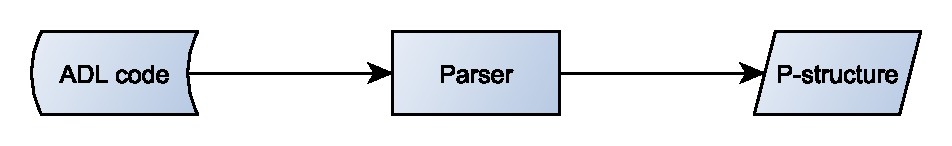
\includegraphics[width=0.5\textwidth]{Architecture}
  \caption[Architecture of the project]{Architecture of the project, showing where the parser fits in the Ampersand system}
\end{figure}

\subsection{Critical success factors}
\subsection{Our objectives and commitments towards the project and customer}

\section{Knowledge acquisition (-)}
\label{sec:knowledge-acquisition}
\subsection{Research context}
Some ideas by Bastiaan:
\begin{itemize}
  \item more info on ampersand users
  \item user-friendly error messages (specific to compilers or not)
  \item parser-libraries
  \item Stef's research (3a)
  \item Haskell parsers (e.g. Helium), monadit or combinators
\end{itemize}

\subsection{Domain \& technology}
\subsubsection{Part Daniel}
\lipsum[1]

\subsubsection{Part Maarten}
\lipsum[1]

\subsection{Knowledge documentation}
\lipsum[1]

\section{Project approach (-)}
\label{sec:project-approach}
\subsection{Project methodology}
\lipsum[1]

\subsection{Project planning}
Milestones \& phases

\subsection{Project milestones and corresponding deliverables }
\lipsum[1]

\section{Project management (M)}
\label{sec:project-management}
\subsection{Project governance / roles \& responsibilities}
\lipsum[1]
\subsection{Communication}
\lipsum[1]
\subsubsection{Internal}
\lipsum[1]
\subsubsection{OU}
\lipsum[1]
\subsubsection{Customer}
\lipsum[1]
\subsection{Time keeping}
\lipsum[1]
\subsection{Project reporting}
\lipsum[1]
\subsection{Quality assurance}
\lipsum[1]
\subsubsection{Process quality \& monitoring}
\lipsum[1]
\subsubsection{Deliverables quality \& monitoring}
\lipsum[1]

\section{Assumptions and limitations (-)}
\label{sec:assumptions-limitations}
(knowledge/architecture/etc...)

\section{Interferences with other projects (-)}
\label{sec:interferences}
(code conflicts, etc...)

\section{Risk management (M)}
\label{sec:risk-management}
\subsection{Risk identification and qualification}
\subsubsection{Functional risks}
\lipsum[1]
\subsubsection{Technical risks}
\lipsum[1]
\subsection{Risk mitigation plan}
\lipsum[1]

\section{Project realization (-)}
\label{sec:project-realization}
\subsection{Coding conventions}
\lipsum[1]
\subsection{Scrum approach}
\lipsum[1]
\subsection{Validation}
\lipsum[1]

\section{Testing \& Validation (-)}
\label{sec:testing-validation}
\subsection{Test approach}
\lipsum[1]
\subsection{Test methodology}
Will we use student's data? That can be hard to do.

\subsection{Test plan \& Milestones}
\lipsum[1]
\subsection{Test documentation}
\lipsum[1]

\section{Issue management (-)}
\label{sec:issue-management}

\section{Integration \& release (-)}
\label{sec:integration-release}
(acceptation, communication, etc...)

\section{Documentation (-)}
\label{sec:documentation}
\subsection{Documentation plan}
\lipsum[1]
\subsection{Deliverables}
\lipsum[1]

\section{Tools, methodologies and accelerators (R-M)}
\label{sec:tools-methodologies}
\subsection{Collaboration}
\dict{Dropbox}{File hosting service that offers cloud storage, file synchronization, personal cloud, and client software}%
\dict{Git}{A distributed revision control and source code management}%
\dict{GitHub}{Git repository web-based hosting service which offers all of the distributed revision control and source code management (SCM) functionality of Git}%
\dict{Microsoft Office}{Office suite of desktop applications devleoped by Microsoft}%
For the collaboration between the project members, the following tools will be used:
\begin{description}
	\item[Dropbox] For sharing time tracking and other reference documents;
	\item[GitHub] For sharing git repositories of code and documentation;
	\item[Microsoft Office] For writing internal documents, e.g. time tracking;
\end{description}

\subsection{Documentation}
\dict{Haddock}{A software documentation generator for the Haskell programming language}%
\dict{TeXworks}{Graphical user interface for editing and compiling \LaTeX{} documents}%
\dict{LaTeX}{Document preparation system and document markup language for the TeX typeset}%
For writing the documentation, the following tools will be used:
\begin{description}
	\item[Haddock] For annotating documentation on the code;
	\item[TeXworks] For writing and compiling \LaTeX{} documents;
\end{description}

\subsection{Design}
\dict{yEd}{Software for editing graphs}%
For designing the software and its architecture, the following tools will be used:
\begin{description}
	\item[yEd] For creating diagrams and graphs;
\end{description}

\subsection{Development}
\dict{IDE}{Integrated Development Environment}%
\dict{GHC}{Glasgow Haskell Compilation system}%
\dict{Cabal}{Library for managing Haskell builds and packages}%
For software development, the following tools will be used:
\begin{description}
	\item[IDE] No standard integrated development environment will be chosen: the project members are free to use any IDE, e.g. Eclipse, Leksah, Notepad++;
	\item[GHC] The compiler GHC (Glasgow Haskell Compilation System), version 7.8.3, will be used;
	\item[Cabal] For managing Haskell packages and compilation, cabal-install version 1.18.0.5 and Cabal library version 1.18.1.3.
\end{description}

\subsection{Testing}
\dict{Hpc}{Library for checking, recording and displaying code coverage}%
\dict{Sentinel}{Test server for the Ampersand project}%
\dict{QuickCheck}{Library for testing Haskell code}%
Finally, the following tools will be used for testing the software:
\begin{description}
	\item[Hpc] might be used for checking, recording and displaying the code coverage of tests;
	\item[Sentinel server] can be used for the integration tests;
	\item[QuickCheck] for automating tests on the code and property based testing (e.g. pretty-print and reparsing, random code generation);
\end{description}

% Appendices
\newpage
\appendix
\addcontentsline{toc}{part}{Appendices}
\label{sec:glossary}
% To update this section, it's necessary to run the file build.bat!
\printglossary[style=altlist,title=Glossary]

\end{document}